\everymath{\displaystyle}

\chapter{Ứng Dụng Convolutional Neural Network Vào Bài Toán Nhận Diện Biển Báo Giao Thông }
\label{chap:chap5}
\section{Dữ liệu}
\subsection{Thông tin dữ liệu}
\hspace{5mm}Dữ liệu được sử dụng trong tài liệu này là German Traffic Sign Recognition Benchmark (GTSRB) có hơn 50000 ảnh được chia ra 43 loại biển báo giao thông. 
\begin{figure}[H]
\begin{center}
\label{fig:data_sample}
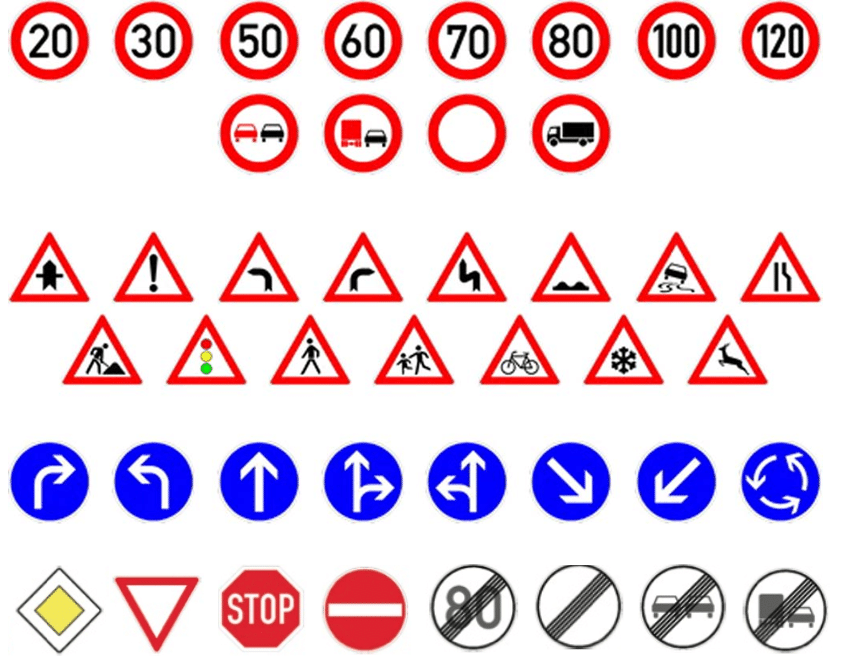
\includegraphics[scale=0.5]{chap5/image/data_sample.png}
\caption{Danh sách các loại biển báo}
\end{center}
\end{figure}
Trong 50000 ảnh biển báo giao thông, có gần 40000 ảnh được dùng trong quá trình huấn luyện, hơn 12000 dùng để kiểm tra và kích thước ảnh được trải từ $15\times 15$ đến $250\times250$ pixels và có định dạng file là '.ppm'. Biển báo abc có nhiều số lượng nhiều nhất là x ảnh, biển báo có lượng ít nhất abc với y ảnh.
\begin{figure}[H]
\begin{center}
\label{fig:data_sample}
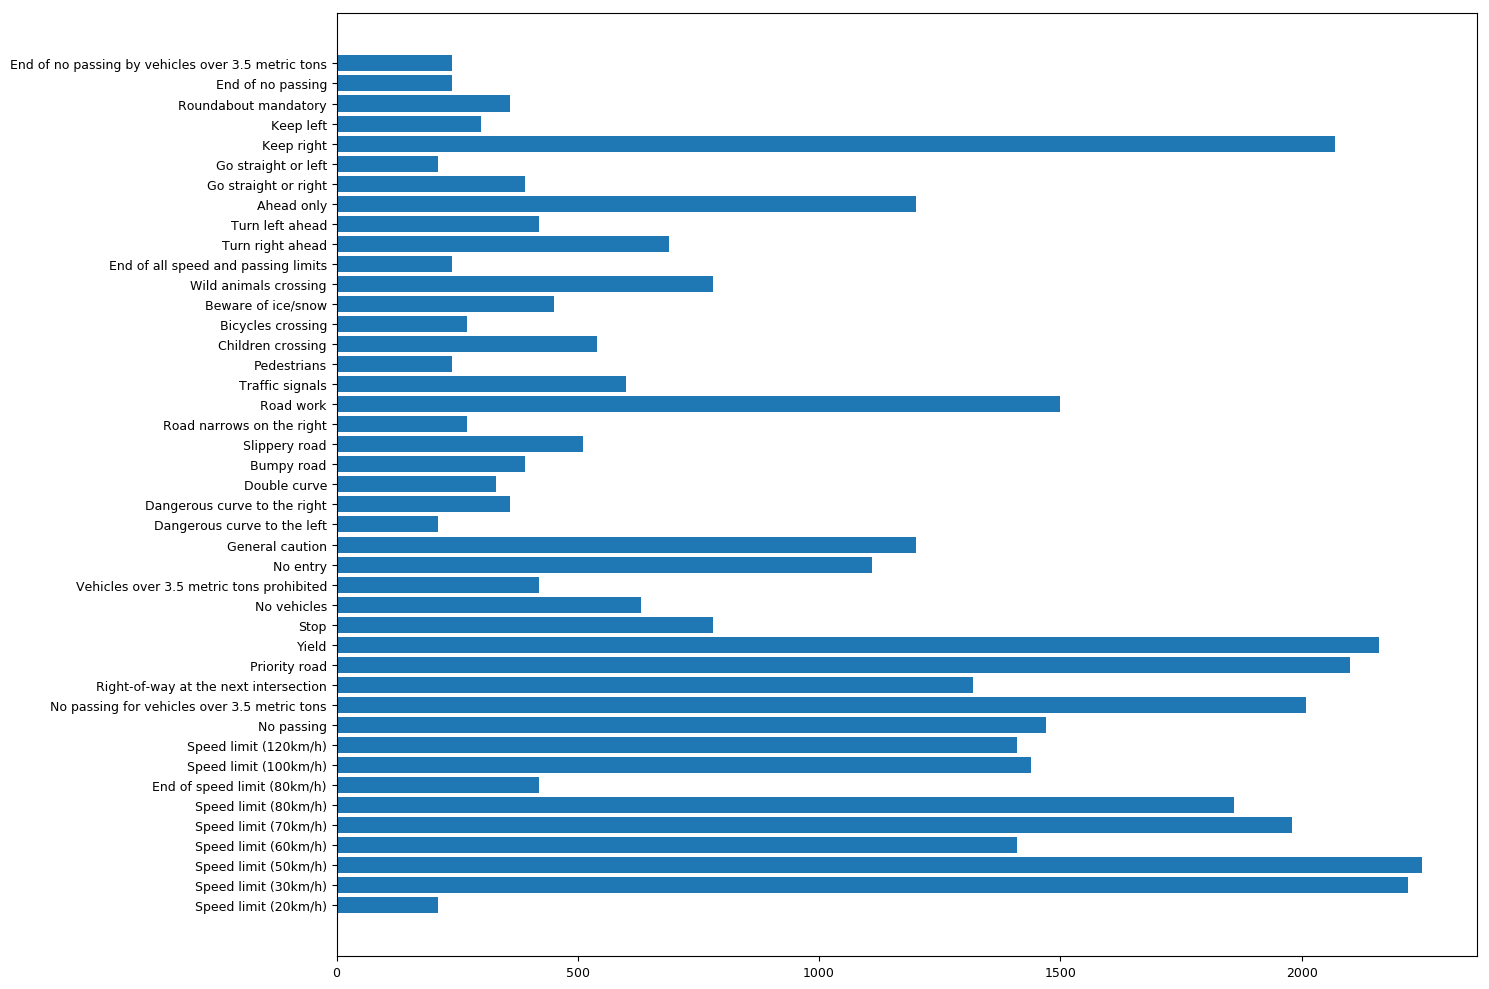
\includegraphics[scale=0.3]{chap5/image/data_statistic.png}
\caption{Thống kê dữ liệu huấn luyện}
\end{center}
\end{figure}
%\textbf{Tổ chức dữ liệu}\par
Dữ liệu được chia làm hai thư mục chính: thư mục chứa tập dữ liệu huấn luyện và thư mục chứa dữ liệu kiểm tra. Trong thư mục dữ liệu huấn luyện, dữ liệu được phân chia thành 43 thư mục con tương ứng với các loại biển báo và được đánh số từ 0 đến 42, trong mỗi thư mục con này là các ảnh của biển báo tương ứng và một file csv chứa tên đầy đủ của file ảnh và nhãn của nó. Trong thư mục dữ liệu kiểm tra sẽ là các dữ liệu không xuất hiện trong tập huấn luyện và một file lưu thông tin giống như ở trong tập huấn luyện.
\subsection{Tăng cường dữ liệu}
\hspace{5mm} Do dữ liệu chúng ta bị mất cân bằng vì thế chúng ta sẽ tạo ra thêm dữ liệu từ dữ liệu ban đầu. Đối với các loại biển báo có ít mẫu dữ liệu, tôi sử dụng một số phương pháp như: xoay ảnh, phóng to, thu nhỏ, dịch chuyển,... sao cho số lượng mẫu giữa các loại biển báo tương đương nahu và tương đương với lớp có số lượng mẫu dữ liệu lớn nhất.
\subsection{Chuẩn hóa dữ liệu}
Tất cả dữ liệu sẽ được chuyển về ảnh với format là gray và kích thước là $32 \times 32$ pixels.